\documentclass[12pt]{article}
\usepackage[magyar]{babel}
\usepackage{t1enc}
\usepackage{graphicx}
\usepackage{enumitem}
\usepackage[headheight=20pt]{geometry}
\usepackage{fancyhdr}
\usepackage[colorlinks,linkcolor=black,%
urlcolor=blue,citecolor=orange,linktoc=all]{hyperref}

\pagestyle{fancy}
\fancyhf{}
\fancypagestyle{plain}{%
\fancyhf{}%
\fancyhf[CH]{Beadandó}%
\fancyhf[LH]{Adatbázisrendszerek I}%
\fancyhf[RH]{Sindely Richárd - P1UV07}%
\fancyhf[CF]{Miskolci Egyetem}%
\fancyhf[RF]{\thepage}%
}
\renewcommand{\footrulewidth}{0.4pt}
\fancyhf[CH]{Beadandó}
\fancyhf[LH]{Adatbázisrendszerek I}
\fancyhf[RH]{Sindely Richárd - P1UV07}
\fancyhf[CF]{Miskolci Egyetem}
\fancyhf[RF]{\thepage}

\author{Sindely Richárd-P1UV07}
\title{Adatbázisrendszerek I. beadandó}
\date{2023}

\begin{document}
\maketitle
\newpage
\tableofcontents
\newpage
\section{Bevezetés}
\label{bev}
Az adatbázisomhoz a volánbusz rendszere adott inspirációt, amelyben van egy \textbf{Utas} egyed, amely a következő tulajdonságokkal rendelkezik:
\begin{itemize}
\item uid (PK - Elsődleges kulcs)
\item név (Az utas neve)
\item szülév (Utas születési éve)
\item személyi ig. szám (Az utas szemlyi ig. száma)
\item telefonszám (Utas telefonszáma)
\item kor (Leszármoztatott érték)
\item jegy/bérlet típusa
\end{itemize}
A következő egyed a \textbf{Busz} ami egy adott buszról tartalmaz információkat.
\begin{itemize}
\item bid (PK - Elsődleges kulcs)
\item rendszám (Busz rendszáma)
\item típusszám (Busz típus/gyártási száma)
\item márka (Busz gyártója)
\end{itemize}
Az \textbf{Utas} és a \textbf{Busz} egyedek között van egy kapcsolat ami tartalmaz egy tulajdonságot ami a:
\begin{itemize}
\item ülés (Ülés száma ahova az utas ül)
\end{itemize}
Van még egy \textbf{Söfőr} egyed ami a céghez tartozó buszsöfőröket tartja számon, melynek a tulajdonságai a következők:
\begin{itemize}
\item sid (PK - Elsődleges kulcs)
\item név (Söfőr neve)
\item kezdés éve (Az év amikor a söfőr elkezdett dolgozni a cégnél)
\item ledolgozott évek száma (Leszármoztatott érték)
\end{itemize}
Következő egyed az a \textbf{Járatszám} ami a következő tulajdonságokkal rendelkezik:
\begin{itemize}
\item jid (PK - Elsődleges kulcs)
\item szam (Járatnak a száma)
\end{itemize}
A \textbf{Megállók} egyed a következő tulajdonságokkal bír:
\begin{itemize}
\item mid (PK - Elsődleges kulcs)
\item koordináta (Megálló helyzetének koordinátája)
\item név (Megálló neve)
\end{itemize}
A \textbf{Járatszám} és a \textbf{Megállók} egyedek között van egy kapcsolat ami kettő tulajdonságot is tartalmaz:
\begin{itemize}
\item tervezett indulás
\item tervezett érkezés
\end{itemize}
Végül a \textbf{Települések} egyed tartalmazza a települések tulajdonságait amelyek a következők:
\begin{itemize}
\item tid (PK - Elsődleges kulcs)
\item irányítószám (Települések irányítószáma)
\item név (Települések neve)
\end{itemize}
\newpage
\section{ER diagram}
Előzőleg bemutatott egyedek, tulajdonságok ER diagrammja:\\
\\
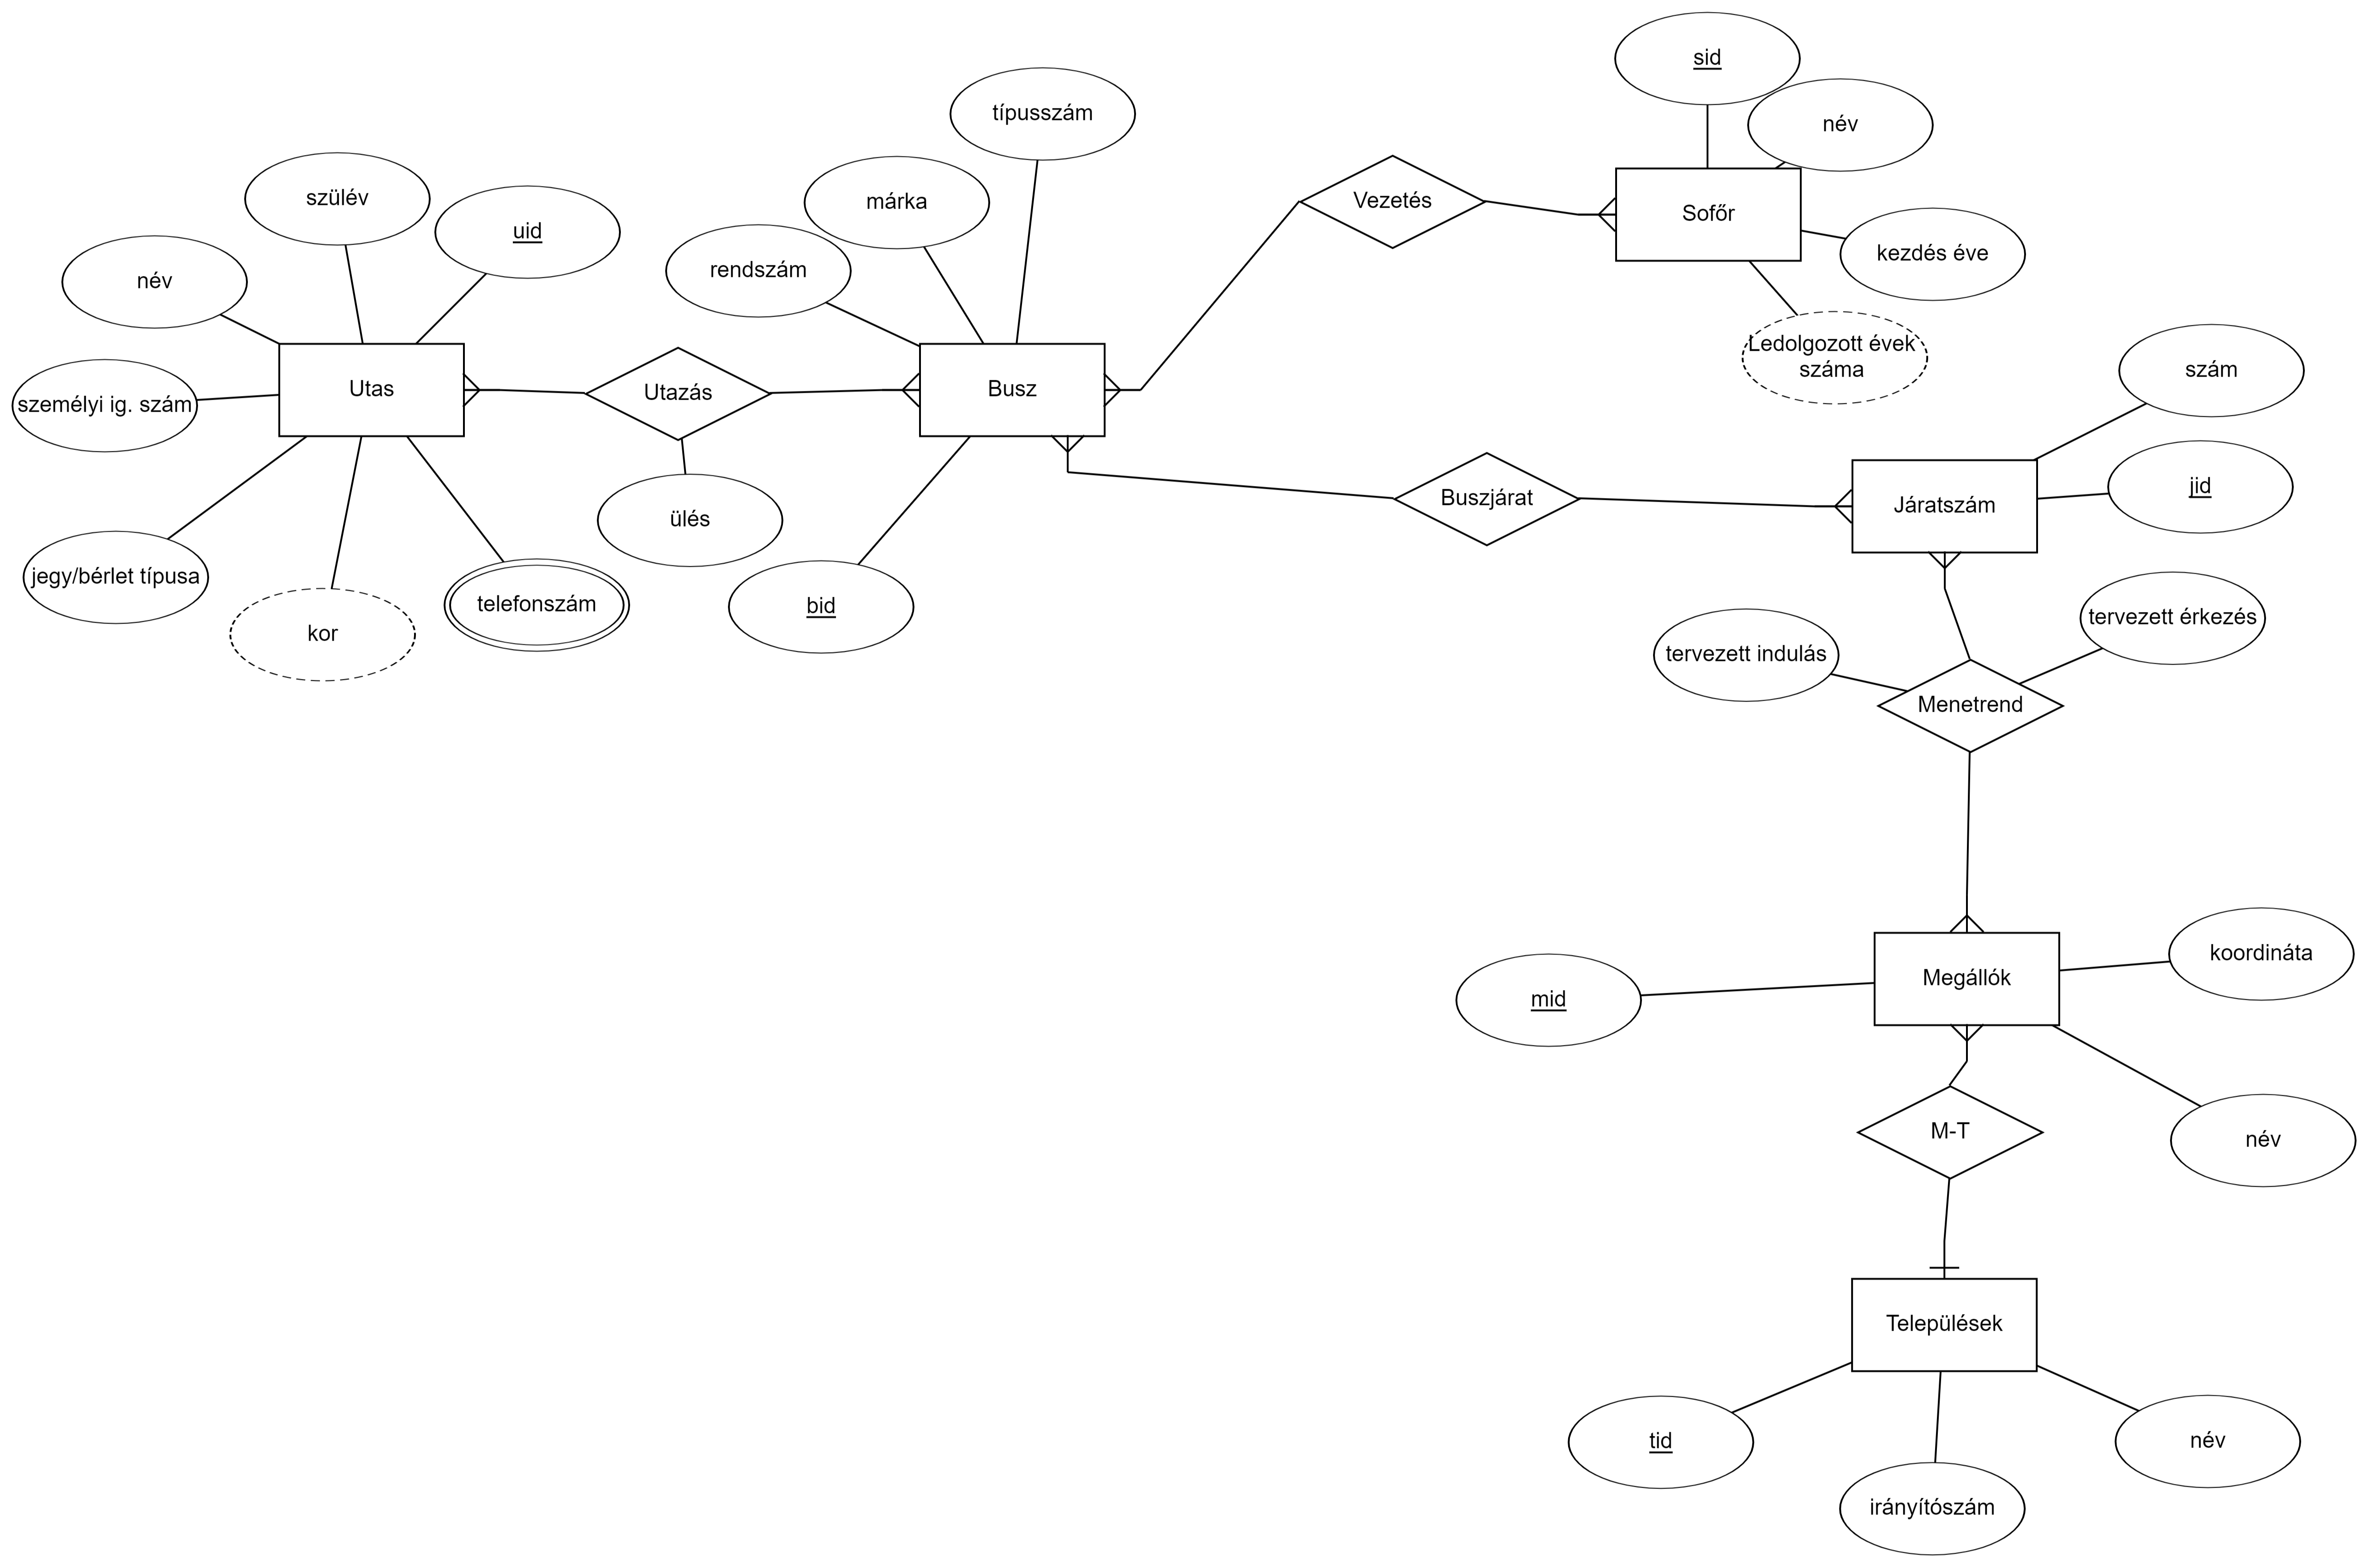
\includegraphics[height=15cm,width=15cm]{D:/Uni/Tex/Adatbázis beadandó/er.png}
\newpage
\section{RS diagram}
Bevezetésben bemutatott egyedek, tulajdonságok RS diagramja:\\
\\
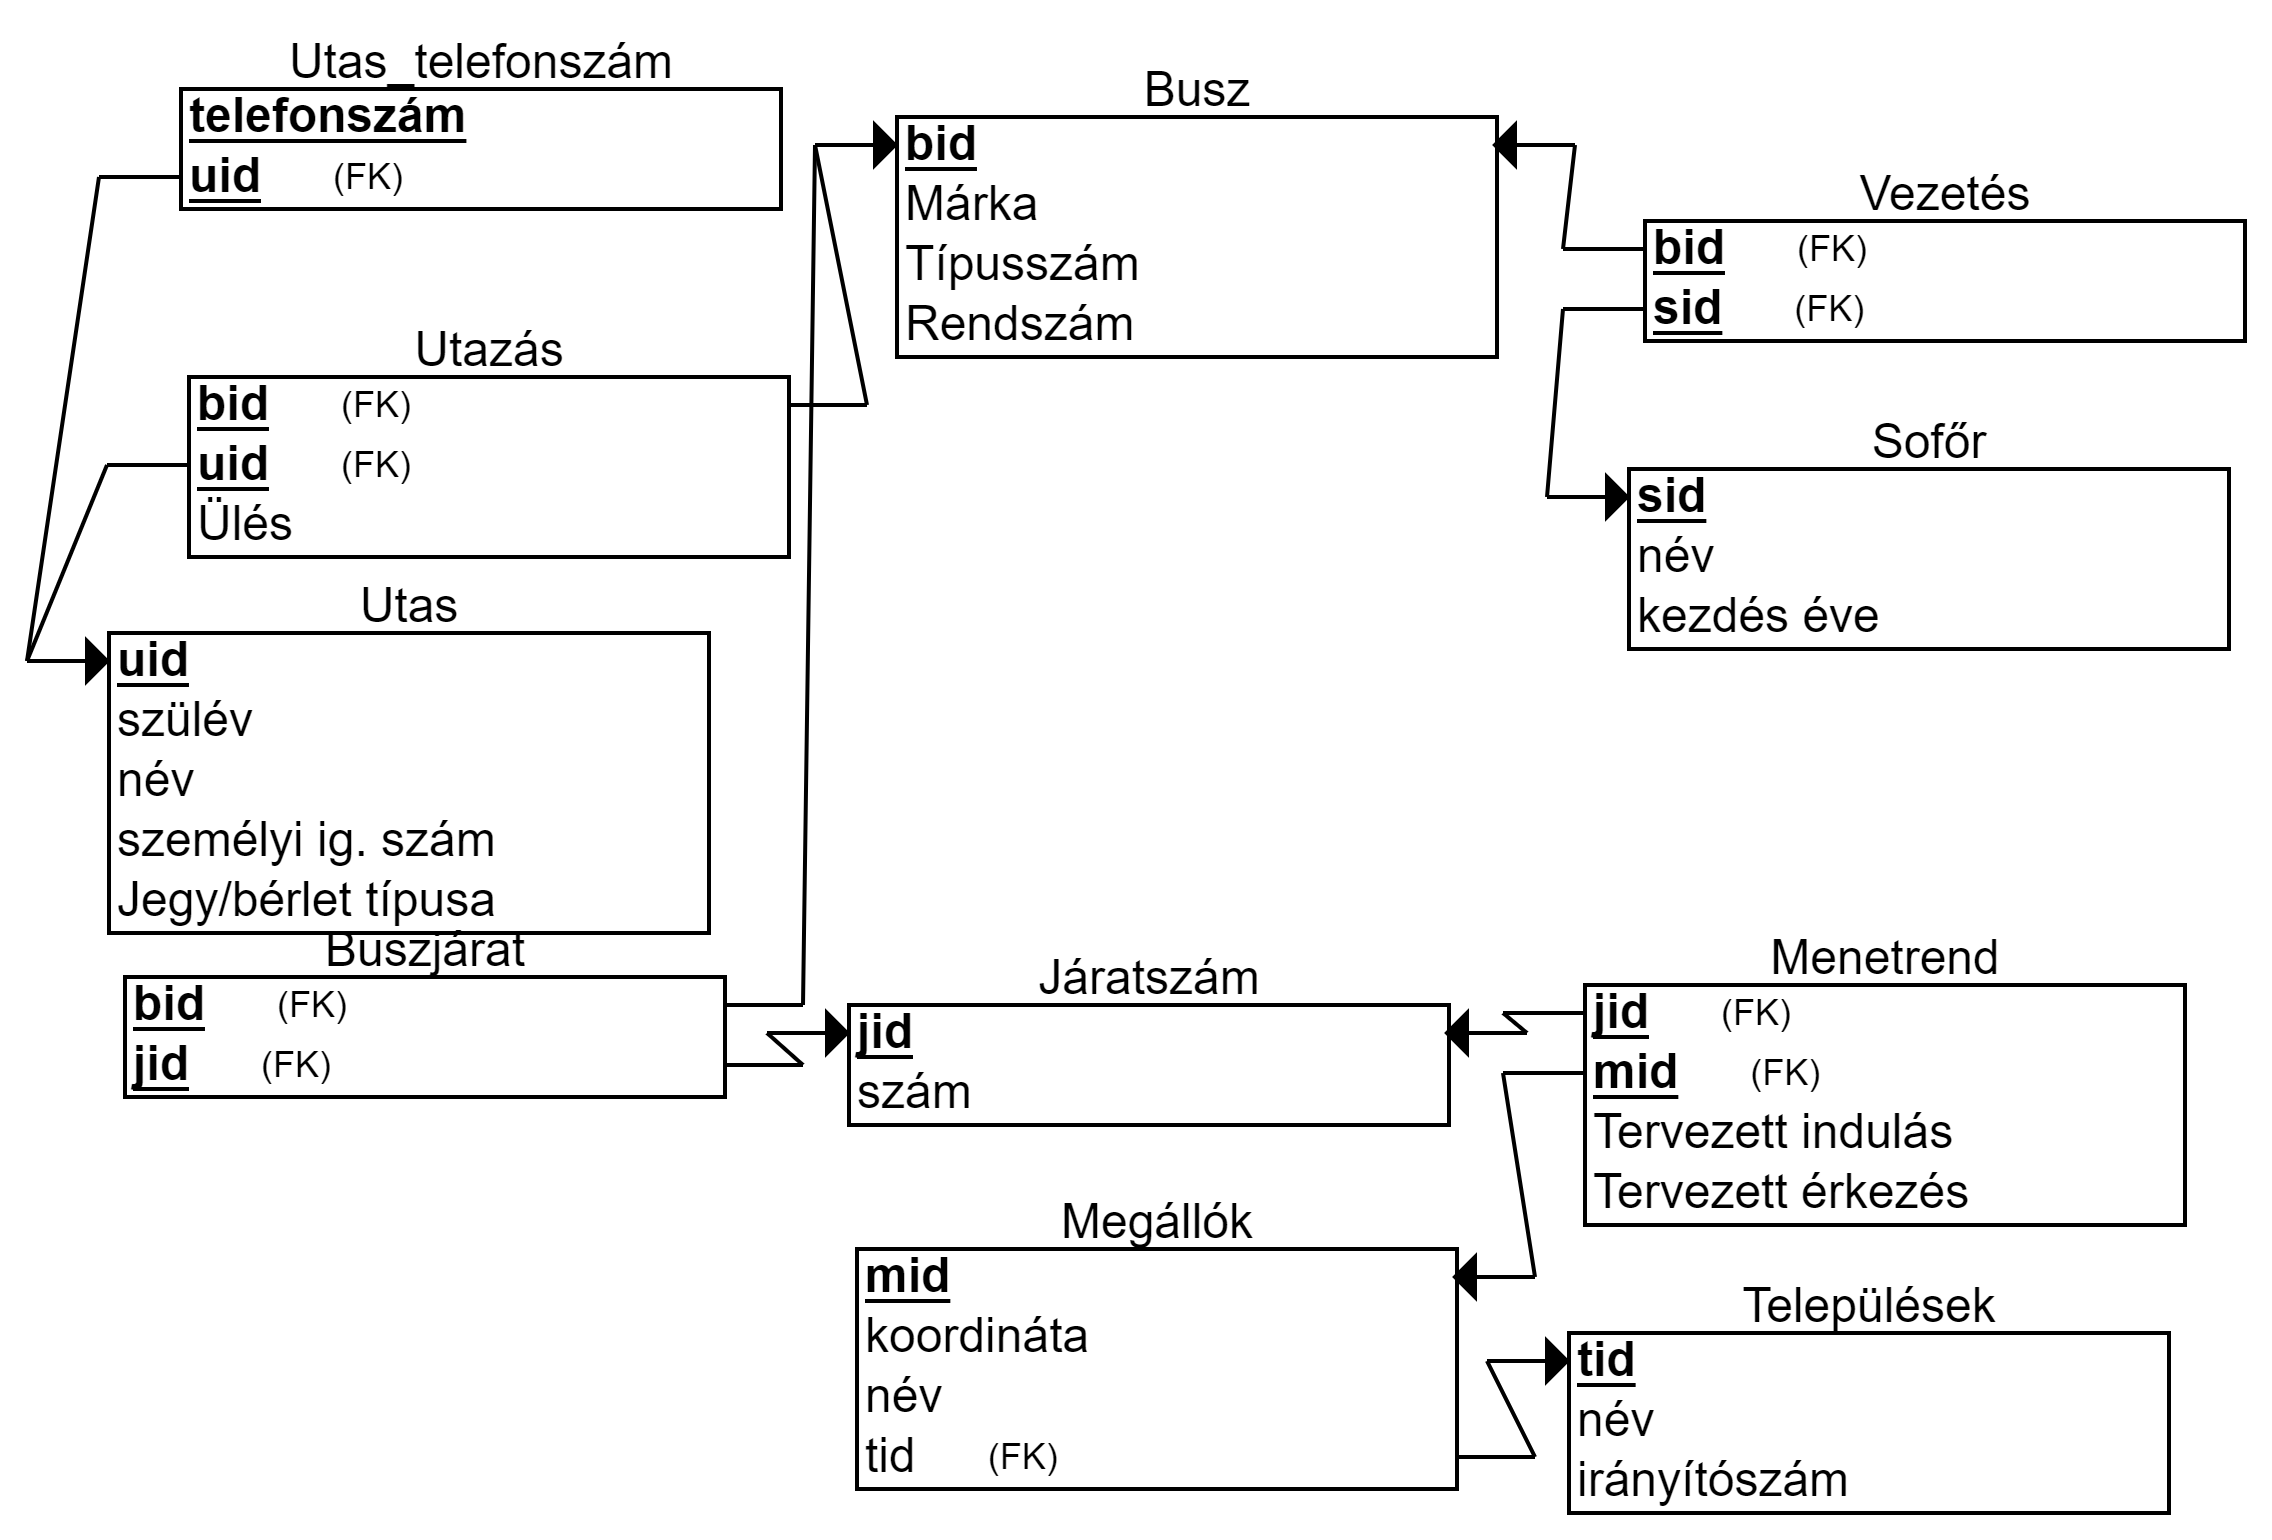
\includegraphics[height=10cm,width=15cm]{D:/Uni/Tex/Adatbázis beadandó/rs.png}
\end{document}